\chapter{Implementarea Sistemelor de Fișiere}

\section{Simularea disk-ului}

\subsection{Initierea disk-ului}

Pentru a putea simula hard disk-ul, vom crea un folder în cadrul sistemului de fișiere oferit de sistemul de operare pe care vor fi rulate mai apoi cele 3 sisteme de fișiere. Acest folder conține 2 fișiere simple, fără extensie: un fișier 'Metadata', care oferă informațiile necesare inițierii simulării (cum ar fi numarul de sectoare ale hard disk-ului si dimensiunea in bytes a fiecarui sector), odată ce aceasta a fost deja creată într-o dată anterioară, și un alt fișier 'Data', care reprezintă disk-ul simulat. Acest fișier este în esență doar un șir de caractere, care vor reprezenta byții din cadrul hard disk-ului nostru simulat.

Pentru crearea celor două fișiere, precum și pentru scrierea și citirea acestora, a fost necesară utilizarea API-ului oferit de sistemul de operare în cadrul căruia este dezvoltată această lucrare de licență, și anume Windows 10. Acesta ne pune la dispoziție o serie de metode pentru manipularea fișierelor, prin intermediul bibliotecii "windows.h".

\bigskip

\begin{figure}[h]
    \centering
    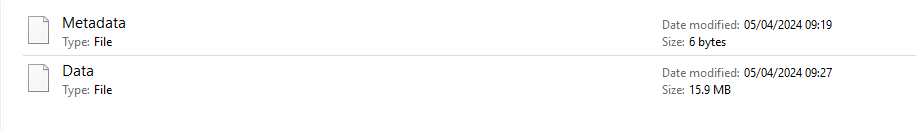
\includegraphics[width=1.0\linewidth]{images/2.1.png}
    \caption{Disk-ul simulat}
    \label{fig:enter-label}
\end{figure}

În momentul în care este creat disk-ul, acesta nu conține nicio informație, toți byții fiind setați la 0. Pentru a realiza acest lucru în cadrul simulării, după crearea celor două fișiere, vom umple fișierul 'Data' cu caracterul null (adică valoare 0), în conformitate cu dimensiunea disk-ului, și anume (numărul de sectoare) * (dimensiunea unui sector). Aceste valori vor fi oferite ca și input de către utilizator la crearea disk-ului, împreună cu locația unde se dorește salvarea simulării acestuia.


\begin{figure}[h]
    \centering
    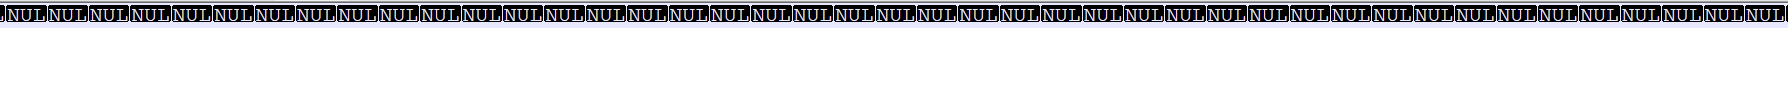
\includegraphics[width=1.0\linewidth]{images/2.2.png}
    \caption{Vizualizare a disk-ului după creare}
    \label{fig:enter-label}
\end{figure}


\subsection{Scrierea si citirea sectoarelor}

Pe lângă crearea și inițierea disk-ului, biblioteca pe care o cream pune la dispoziție, în mod evident și o serie de funcții care ajută la scrierea și citirea datelor aflate pe disk. Scrierea și citirea byte-ilor a fost realizată într-un mod care să simuleze felul în care datele sunt extrase și modificate de pe un disk real, bineînțeles cu limitările pe care ni le impune faptul că în realitate lucrăm cu un fișier aflat în cadrul sistemului de operare Windows 10, și nu cu o componentă hardware adevărată. Astfel, fiecare operațiune de scriere sau citire afectează întregul conținut al unui sector, sau a mai multor sectoare consecutive.

Să luăm ca și exemplu, un disk care are dimensiunea sectoarelor de 512 bytes. În cazul în care dorim să citim byții aflați între adresele 800 și 1200, noi vom citi de fapt toți byte-ii de la adresa 512 până la 1535, adică sectoarele 1 și 2 în totalitate (indexarea sectoarelor făcându-se de la 0), același lucru întâmplându-se și în cazul operației de scriere.

\bigskip

\lstset{style=code-snyppet-style}
\begin{lstlisting}
static int readSector(DiskInfo *diskInfo, uint32_t sector, char *buffer)
{
    char *fullFilePath = buildFilePath(diskInfo->diskDirectory);

    HANDLE fileHandle = CreateFile(fullFilePath,OFN_READONLY,0,nullptr,
                          OPEN_EXISTING, FILE_ATTRIBUTE_NORMAL,nullptr);

    if(fileHandle == INVALID_HANDLE_VALUE)
    {
        CloseHandle(fileHandle);
        delete[] fullFilePath;
        return SECTOR_READ_FAILED;
    }

    OVERLAPPED overlapped;
    memset(&overlapped, 0, sizeof(OVERLAPPED));
    overlapped.Offset = diskInfo->diskParameters.sectorSizeBytes * sector;
    overlapped.hEvent = nullptr;

    DWORD dwBytesRead = 0;
    bool readFileResult = ReadFile(fileHandle, buffer, 
        diskInfo->diskParameters.sectorSizeBytes, &dwBytesRead, &overlapped
        );

    if(!readFileResult || dwBytesRead < diskInfo->diskParameters.sectorSizeBytes)
    {
        CloseHandle(fileHandle);
        delete[] fullFilePath;
        return SECTOR_READ_FAILED;
    }

    CloseHandle(fileHandle);
    delete[] fullFilePath;

    return SECTOR_READ_SUCCESS;
}
\end{lstlisting}

\subsection{Probleme intâmpinate}

Ideea din spatele acestei simulări a fost încă de la început aceea de a putea fi folosită, într-un stil similar, de toate cele 3 sisteme de fișiere care vor fi implementate folosindu-se de funcționalitățile oferite de aceasta. Astfel, în momentul finalizării librăriei, aceasta a trebuit să pună la dispoziție o interfață care urma să fie folosită în cadrul celor 3 proiecte, fără a mai fi modificată ulterior, pentru a nu trebui să facem modificări în cadrul sistemelor de fișiere, datorită faptului că simularea disk-ului a suferit schimbări (adică s-a dorit ca toate modificările ulterioare să fie backwards compatible). Mai jos se poate vedea API-ul pus la dispoziție de către  librărie, acesta nesuferind nicio modificare ulterioară de-a lungul dezvoltării acestei lucrări de licență.

\bigskip

\lstset{style=code-snyppet-style}
\begin{lstlisting}
DiskInfo* initializeDisk(const char* diskDirectory, uint32_t sectorsNumber, uint16_t sectorSize);

int fillDiskInitialMemory(DiskInfo *diskInfo, uint32_t batchSize);

DiskInfo* getDisk(const char* diskDirectory);

int getDiskStatus(DiskInfo *diskInfo);

int readDiskSectors(DiskInfo *diskInfo, uint32_t numOfSectorsToRead, uint32_t sector, char* buffer, uint32_t &numOfSectorsRead);

int writeDiskSectors(DiskInfo *diskInfo, uint32_t numOfSectorsToWrite, uint32_t sector, char buffer[], uint32_t &numOfSectorsWritten);
\end{lstlisting}

\bigskip

Deși această interfață a fost gândită astfel încât să nu necesite modificări ulterioare, asta nu înseamnă că implementarea sa nu a trecut prin anumite schimbări de-a lungul timpului. Pe lângă mici bug-uri care au fost reparate, cum ar fi ștergerea unui pointer null, sau dealocarea la momentul inoportun a unui buffer folosit la scrierea/citirea datelor, a fost necesară și o regândire totală a modului în care sectoarele sunt definite în cadrul simulării.

Așa cum am văzut mai sus, în momentul actual disk-ul în sine, este simulat cu ajutorul unui singur fișier 'Data', care conține toți byții din cadrul său, sectoarele nefiind separate în mod 'fizic' în interiorul acestui fișier, distincția dintre ele făcându-se doar la nivel logic. Acesta nu a fost însă cazul încă de la început, implementarea inițială presupunând existența unui fișier separat pentru fiecare sector în parte.

\bigskip

\begin{figure}[h]
    \centering
    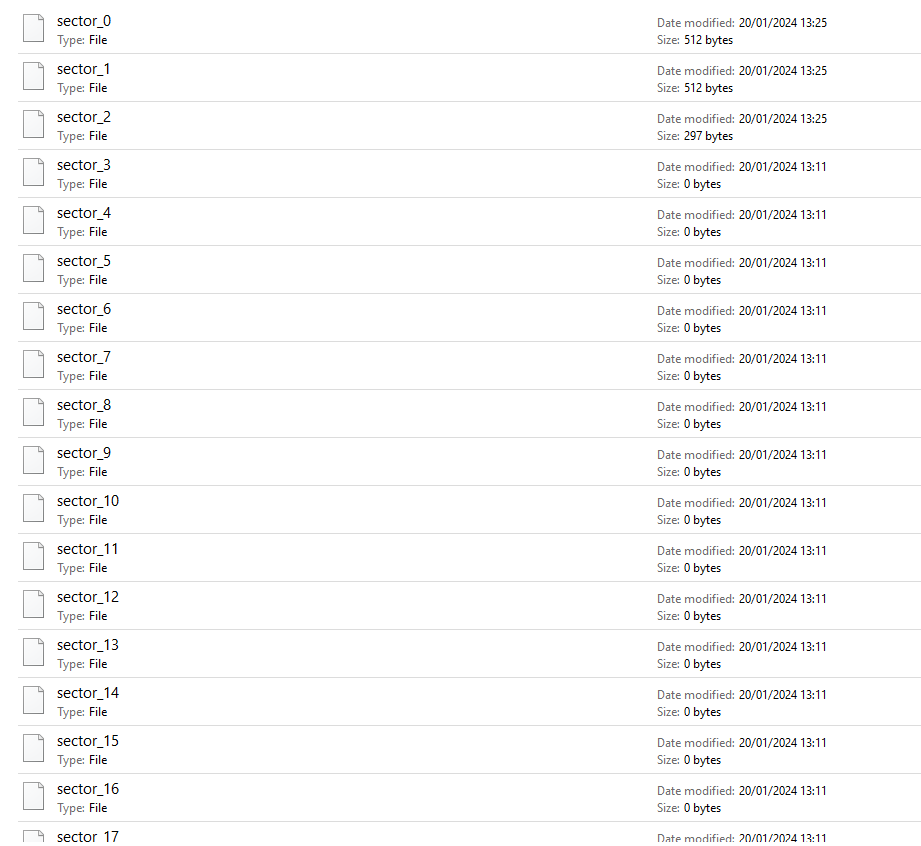
\includegraphics[width=1.0\linewidth]{images/2.3.png}
    \caption{Implementarea inițială a disk-ului}
    \label{fig:enter-label}
\end{figure}

\bigskip

De ce am făcut această schimbare drastică? Ei bine, în timpul dezvoltării primului dintre cele 3 sisteme de fișiere, și anume FAT32, am observat probleme legate de timpul necesar creării hard disk-ului. Inițial am ignorat acest lucru, întrucât în cadrul dezvoltării erau suficiente disk-uri de dimensiuni reduse (512 KiB) pentru testele pe care le făceam, astfel și timpul inițierii fiind unul redus, însă odată cu evoluția implementării, teste pe fișiere de dimensiuni mai ample au devenit necesare, astfel și dimensiunea disk-ului trebuind să crească în mod corespunzător. În acest moment, problemele legate de performanța instantierii disk-ului au devenit tot mai vizibile, devenind chiar un impediment major în procesul de testare. Spre exemplu, crearea unui disk de 1 GiB dura inițial aproximativ 30 de minute, spre deosebire de câteva secunde, cât durează cu implementarea actuală, care folosește un singur fișier, și nu câte unul pentru fiecare sector.

Problemele de performanță, însă, nu erau cauzate doar de existența unui număr ridicat de fișiere, ci și a modului în care se realiza popularea inițială a datelor din cadrul disk-ului, cu caracterul null (valoarea 0).

\bigskip

\lstset{style=code-snyppet-style}
\begin{lstlisting}
int fillDiskInitialMemory(DiskInfo *diskInfo, uint32_t batchSize);
\end{lstlisting}

\bigskip

Astfel, au existat 3 moduri de 'umplere' a disk-ului, până să se ajungă la varianta finală, care este bineînțeles și cea mai eficientă.

\begin{itemize}
  \item \textbf{Popularea fiecărui fișier ce constituia un sector}, aceasta fiind varianta folosită în cadrul implementării inițiale, care folosea câte un fișier separat pentru reprezentarea fiecărui sector, și astfel, scrierea acestora făcându-se în mod independent.
  
  \item \textbf{Popularea independentă a fiecărui sector logic}, aici vorbim deja de cea de-a doua implementare a disk-ului, care folosește un singur fișier, și unde sectoarele sunt separate doar la nivel logic. Cu toate acestea, popularea fiecărui sector se realiza separat, acest lucru presupunând un număr ridicat de operațiuni de deschidere, scriere și apoi închidere asupra fișierului 'Data', ceea ce ducea la o performanță scăzută.
  
  \item \textbf{Popularea sectoarelor în batch-uri}, această variantă finală presupune exploatarea faptului că sectoarele nu sunt separate în mod fizic, ci sunt poziționate consecutiv în interiorul fișierului 'Data'. Astfel, pentru a reduce numărul operațiunilor asupra acestui fișier, popularea lor se realizează în batch-uri de mai multe sectoare.
  
\end{itemize}














\newpage

\section{FAT32}

\subsection{Privire de ansamblu asupra FAT32}

FAT32 este un sistem de fișiere relativ simplu, care presupune utilizarea unei tabele de indici (File Allocation Table) pentru înlănțuirea unor blocuri de date numite clustere. Din punct de vedere structural, FAT32 se împarte în 4 regiuni:

\begin{itemize}
  \item \textbf{Reserved area}, această zonă conține date necesare pentru pornirea și funcționarea sistemelor din cadrul calculatorului. În prima parte a acestei regiuni se află 'Boot Record', care conține codul ce trebuie executat inițial pentru pornirea sistemului, totodată aici aflându-se o serie de structuri de date necesare sistemului nostru de fișiere, și anume Bios Parameter Block (BPB), Extended Boot Record (EBP) și FSInfo.
  
 \item \textbf{FAT 1}, regiune ce reprezintă tabela de indici menționată mai sus. Aceasta conține o serie de valori de 32 de biți (dintre care doar ultimii 28 sunt luați în considerare, primii 4 fiind ignorați), fiecare astfel de valoare reprezentând numărul următorului cluster în cadrul înlănțuirii actuale (a directorului curent). Spre exemplu, dacă la indexul 16 (adică byte-ul 64) se află valoarea 783, înseamnă că datele aflate în continuarea celor din cluster-ul 16 se află în cluster-ul 783.
 
 \item \textbf{FAT 2}, este o copie a FAT 1, servind în special ca și un backup, în cazul posibilelor erori ce pot apărea în tabela principală.
 
 \item \textbf{Data Area}, această regiune conține datele propriu-zise, înglobând folderele și fișierele stocate. Prima parte a acestei zone este numită 'Root directory', și se comportă ca un director obișnuit, acesta putând conține atât sub-foldere cât și fișiere. Aspectul distinctiv al acestuia însă, este faptul că este singurul director ce nu are un părinte, el reprezentând rădăcina arborelui de directoare stocate în cadrul sistemului de fișiere.  
\end{itemize}


\begin{figure}[h]
    \centering
    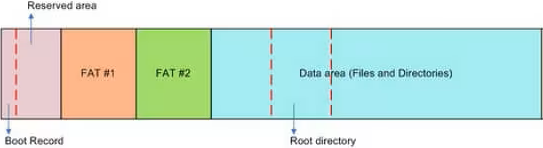
\includegraphics[width=1.0\linewidth]{images/2.4.png}
    \caption{Structura FAT32}
    \label{fig:enter-label}
\end{figure}

\bigskip


\subsection{Modul de implementare}

Fiind în esență doar o simulare (la fel ca toate cele 3 sisteme de fișiere din cadrul acestei lucrări), implementarea FAT32 a trebuit adaptată astfel încât să funcționeze fără a avea acces la hardware, ci doar la discul nostru simulat, și fără a face parte dintr-un sistem de operare. Singura interacțiune de acest fel este una indirectă, prin intermediul simulării discului, atunci când se realizează operațiuni asupra datelor stocate de acesta.

Din aceste considerente, simularea de FAT32 rulează sub forma unui program, cu care utilizatorul poate interacționa prin intermediul terminalului. Așa cum am precizat și mai sus, simularea noastră nu are legătură în mod direct cu sistemul de operare, ca în cazul unui sistem de fișiere adevărat. Aceasta duce la imposibilitatea ca structurile de date de care avem nevoie în cadrul FAT32 să se afle în mod permanent în memorie (RAM), și totodată la lipsa unor procese special dedicate care să ruleze în momentul în care se dorește realizarea unei operațiuni asupra disk-ului (cum ar fi scrierea sau citirea datelor). De aceea, am considerat ca rularea programului de simulare este singura soluție viabilă in cazul nostru.


\subsubsection{Inițializarea FAT32}

În momentul în care programul este rulat, acesta parcurge mai multe etape in vederea pregatirii disk-ului, cat si a sistemului de fisiere propriuzis:

\begin{enumerate}
  \item \textbf{Verificarea existenței disk-ului}, aici se verifică dacă disk-ul a fost deja inițializat la locația dată ca și parametru.

  \item \textbf{Initializarea/Citirea disk-ului}, această etapă depinde de rezultatul pasului anterior. Dacă simularea disk-ului nu a fost găsită la locația precizată, acesta este instantiat: se creează fișierele 'Metadata' și 'Data', acesta din urmă fiind populat cu null (valoarea 0), în conformitate cu dimensiunea dorită. Dacă disk-ul a fost deja inițiat, atunci se citesc datele referitoare la acesta și se stochează într-o structură de date, DiskInfo, care ne va fi de folos pe parcurs.

  \item \textbf{Verificarea inițializării sistemului de fișiere}, acest pas realizează citirea primului sector de pe disc, adică a sectorului de bootare. Dacă la finalul acestui sector se află semnătura specifică sistemului de fișiere FAT32, și anume 0xAA55, înseamnă că sistemul a fost deja inițiat, altfel, nu.

  \item \textbf{Inițializarea sistemului de fișiere}, etapă ce are loc doar în cazul în care verificarea de mai devreme returnează fals. În cadrul acestui pas sunt create datele din cadrul BIOS Parameter Block (BPB) și a Extended BIOS Parameter Block (EBPB), care vor fi stocate împreună în cadrul unei structuri numite BootSector, pentru ca mai apoi să fie salvate în sectorul de bootare (sectorul 0), bineînțeles împreună cu semnătura reprezentativă FAT32 despre care am vorbit mai sus. Tot aici este creată o altă structură de date, FSInfo, aceasta fiind salvată în sectorul 1. De asemenea, sunt salvate și câteva date esențiale referitoare la Directorul Radăcină (cum ar fi dimensiunea, primul cluster etc.), în cadrul intrării 'dot' a acestuia.

  \item \textbf{Citirea structurilor de date necesare}, indiferent de rezultatul de la pasul anterior, citim structurile BootSector si FSInfo de pe disk.

  \item \textbf{Inițializarea tabelelor de indici}, această etapă se realizează doar în cazul în care sistemul de fișiere a fost inițiat anterior (la pasul 4). Specificația FAT32 precizează faptul că Zona de Date începe întotdeauna de la cluster-ul numărul 2, de aceea setăm în tabelul de indici primele 2 clustere ca fiind rezervate, iar cel de-al treilea (care aparține Directorului Radăcină) ca fiind cluster final în cadrul înlănțuirii.
  
\end{enumerate}

\bigskip

\lstset{style=code-snyppet-style}
\begin{lstlisting}
void fat32Startup(char* diskDirectory, DiskInfo** diskInfo, 
                  BootSector** bootSector, FsInfo** fsInfo, 
                  uint32_t sectorsNumber, uint32_t sectorSize)
{
    if(checkDiskInitialization(diskDirectory) == false)
        initializeDisk(diskDirectory, diskInfo, sectorsNumber, sectorSize);
    else
        *diskInfo = getDisk(diskDirectory);

    bool fat32AlreadyInitialized = true;
    if(checkFat32FileSystemInitialization(*diskInfo) == false)
    {
        initializeBootSectors(*diskInfo);
        fat32AlreadyInitialized = false;
        std::cout << "Boot sectors initialized\n";
    }

    *bootSector = readBootSector(*diskInfo);
    *fsInfo = readFsInfo(*diskInfo, *bootSector);

    if(fat32AlreadyInitialized == false)
    {
        initializeFat(*diskInfo, *bootSector);
        std::cout << "File allocation table initialized\n";
    }
}
\end{lstlisting}

\bigskip

\subsubsection{Structura unui director}

Directoarele din cadrul implementării noastre de FAT32 pot fi de 2 tipuri: folder sau fișier. Modul în care acestea sunt stocate în Zona de Date este unul asemănător, însă diferența o face scopul acestora și tipul de date pe care acestea îl pot îngloba. Un lucru comun pe care îl au ambele tipuri de directoare sunt intrările speciale 'dot' și 'dotdot', având lungimea de 4 bytes și aflându-se la începutul fiecărui director. Printre altele, intrarea 'dot' conține valoarea cluster-ului în care se află, în timp ce intrarea 'dotdot' conține valoarea primului cluster al părintelui, astfel acestea ajutând la traversarea arborelui de directoare ce se formează în cadrul sistemului de fișiere.

Datele conținute într-un folder sunt de tipul DirectoryEntry, o structură care are lungimea de 4 bytes și care conține informații referitoare la un director copil, cum ar fi numele său, dimensiunea, valoarea primului cluster sau date temporale. Pentru fiecare urmaș direct al unui director, acesta conține o intrare de acest fel, intrările fiind poziționate consecutiv în cadrul clusterelor. Datele aflate în clusterele corespunzătoare unui folder vor fi interpretate doar sub forma acestor tipuri de intrări, ceea ce înseamnă că un folder nu poate conține și alt tip de date.

\bigskip

\lstset{style=code-snyppet-style}
\begin{lstlisting}
typedef struct
{
    uint8_t FileName[11];
    uint8_t Attributes;
    uint8_t Reserved;
    uint8_t CreationTimeTenths;
    uint16_t CreationTime;
    uint16_t CreationDate;
    uint16_t LastAccessedDate;
    uint16_t FirstClusterHigh;
    uint16_t LastWriteTime;
    uint16_t LastWriteDate;
    uint16_t FirstClusterLow;
    uint32_t FileSize;
} __attribute__((packed)) DirectoryEntry;
\end{lstlisting}

\bigskip

Spre deosebire de foldere, un fișier obișnuit conține numai date simple, care nu sunt interpretate sub nicio formă de către sistemul de fișiere. Ele sunt scrise și citite fără a fi analizate sau modificate în vreun fel.


\subsubsection{Alocarea de clustere}

Fie că dorim să creăm un director sau să extindem unul deja existent, este necesară realizarea unei alocări de clustere, un proces care se desfășoară în mai mulți pași. Alocarea unui nou cluster se realizează atunci când ultimul cluster din cadrul directorului nu mai conține suficienți bytes liberi pentru a încăpea întreaga cantitate de date care se dorește a fi scrisă.

În prima fază, se caută un cluster liber, fără a avea importanță poziția sau vecinii acestuia pe disc. Pentru a realiza această căutare, se parcurge tabelul de indici până când este găsită valoarea 0, reprezentând un cluster liber.

Dacă această căutare are succes, clusterul găsit este marcat în tabelul de indici cu valoarea 0xFFFFFFFF, reprezentând finalul unei înlănțuiri de clustere (END OF CHAIN). În cazul în care acest nou cluster nu este primul din cadrul unui director, trebuie actualizată și valoarea din tabel a precedentului ultim cluster, astfel încât acesta să indice către cel nou.


\subsubsection{Cautarea unui director}

Indiferent ce fel de operație dorim să realizăm asupra unui director, primul pas care trebuie făcut este să-i descoperim locația, mai exact să aflăm care este primul său cluster. Pentru asta, trebuie parcurs arborele de directoare, pornind de la Directorul Rădăcină, până când ajungem la destinația dorită. Astfel, este folosită o funcție recursivă, care iterează prin DirectoryEntry-urile folder-ului curent, în căutarea unui director care să aibă denumirea pe care o căutăm. Odată găsit directorul căutat, putem afla informațiile necesare despre acesta, precum primul său cluster sau dimensiunea sa prin intermediul structurii de date menționate mai devreme.


\subsubsection{Crearea directoarelor}

Crearea unui director, fie că acesta este de tip folder sau fișier obișnuit, este un proces complex, care presupune interacțiunea cu majoritatea funcționalităților din cadrul implementării noastre.

Înainte de începerea instanțierii propriu-zise a acestui nou director, se verifică faptul că datele oferite sunt valide: se verifică dacă numele respectă formatul corespunzător și nu conține caractere interzise, se verifică existența directorului oferit drept părinte, se verifică faptul că acesta este de tipul folder, iar în final ne asigurăm că nu există un alt director cu numele similar celui pe care dorim să-l cream, deoarece duplicarea denumirilor nu este permisă.

Apoi, se caută un cluster disponibil, care este alocat noului director, iar apoi sunt introduse intrările 'dot' și 'dotdot' în prima parte a acestuia. În final, este creat un DirectoryEntry corespunzător și este adăugat în ultimul cluster al părintelui.


\subsubsection{Scrierea fișierelor}

Când vine vorba despre scrierea datelor în fișiere, există 2 moduri prin care putem face acest lucru în cadrul implementării noastre:

\begin{itemize}
  \item \textbf{Modul TRUNCATE}, care presupune suprascrierea byților deja existenți, adăugarea datelor realizându-se începând cu primul byte disponibil, adică byte-ul 64 din cadrul fișierului (primii 64 bytes fiind ocupați de intrările 'dot' și 'dotdot').

  \item \textbf{Modul APPEND}, În acest mod, datele pe care dorim să le scriem sunt adăugate în continuarea celor existente deja, fără a se produce vreo suprascriere, deci fără a suferi vreo pierdere de date.
\end{itemize}

Pentru ca operațiunea de scriere să fie posibilă, fișierul nostru trebuie să aibă alocat un număr suficient de clustere. În cazul scrierii în modul truncate, dacă dimensiunea datelor este mai redusă decât dimensiunea actuală a fișierului, atunci nu mai trebuie adăugate clustere, ci dimpotrivă, este posibil să fie necesară eliberarea unei părți din acestea. În caz contrar, sau în cazul în care operăm în modul append, alocarea de noi clustere este un lucru ce se va întâmpla în cele mai multe situații. După alocarea clusterelor și scrierea datelor, se realizează actualizarea informațiilor despre fișierul actual în DirectoryEntry-ul corespunzător acestuia aflat în părintele său, cât și intrările sale 'dot' și 'dotdot'.


\subsubsection{Citirea fișierelor}

Citirea datelor din cadrul unui fișier se poate realiza atât în totalitate, cât și parțial. Implementarea noastră permite citirea unui anumit număr de bytes, începând de la o poziție de start. Această operațiune se realizează destul de simplu, fiind necesară doar identificarea fișierului dorit, iar apoi parcurgerea clusterelor sale, începând cu poziția inițială dată, până când numărul dorit de bytes a fost citit (sau până când am ajuns la finalul fișierului).


\subsubsection{Eliberarea memoriei fisierelor}

In cazul in care dorim eliminam o parte dintr-un fisier, cu scopul eliberarii spatiului, acest lucru se poate realize prin intermediul unei operatii de truncate. Aceasta se realizeaza prin marcarea ca neocupate in cadrul tabelei de indexi a clusterelor ce se doresc a fi eliberate. 


\subsubsection{Ştergerea directoarelor}

Dacă dorim să ștergem în totalitate un director, lucrurile pot deveni mai complicate. La fel ca și în cazul eliberării memoriei, clusterele trebuie marcate ca ocupate, iar datele referitoare la director trebuie șterse din părintele acestuia. În cazul folderelor, trebuie realizată și ștergerea moștenitorilor direcți, cât și indirecți ai acestora. Pentru acest lucru, se folosește o metodă recursivă, care utilizează un algoritm breadth-first. Acesta începe cu ștergerea 'frunzelor' din cadrul arborelui de directoare și urcă, până se ajunge la folderul a cărui ștergere a fost cerută.


\subsection{Interacțiunea cu utilizatorul}

Pentru a putea interacționa cu sistemul de fișiere, în timpul rulării simulării acestuia, utilizatorul are posibilitatea de a introduce de la terminal o serie de comenzi ce realizează operațiile descrise în detaliu mai sus, până când acesta introduce comanda 'exit' ce semnalează dorința de a închide programul.

\bigskip

\lstset{style=code-snyppet-style}
\begin{lstlisting}
while(true)
    {
        std::cout << '\n';
        std::getline(std::cin, command);

        if(command == "exit")
        {
            std::cout << "Process terminated with exit";
            break;
        }

        std::vector<std::string> tokens = splitString(command, ' ');

        if(tokens[0] == "mkdir")
            commandCreateDirectory(diskInfo, bootSector, tokens);
        else if(tokens[0] == "ls")
            commandListSubdirectories(diskInfo, bootSector, tokens);
        else if(tokens[0] == "write")
            commandWriteFile(diskInfo, bootSector, tokens);
        else if(tokens[0] == "read")
            commandReadFile(diskInfo, bootSector, tokens);
        else if(tokens[0] == "truncate")
            commandTruncateFile(diskInfo, bootSector, tokens);
        else if(tokens[0] == "rmdir")
            commandDeleteDirectory(diskInfo, bootSector, tokens);
        else if(tokens[0] == "la")
            commandShowDirectoryAttributes(diskInfo, bootSector, tokens);
        else
            std::cout << "Unknown command \n";
    }
\end{lstlisting}

\bigskip

Comenzile ce pot fi introduse de la terminal sunt:

\begin{itemize}
  \item \textbf{ls (Nume folder)} sau \textbf{ls -l (Nume folder)}: \textit{ls Root/MyFile} sau \textit{ls -l Root/MyFile} - listează sub-directoarele unui folder, cea de-a doua comandă afișând și dimensiunea acestora.

  \item \textbf{write (Nume fișier) (Număr bytes) (Mod scriere) (Terminator)}: \textit{write Root/MyFile 10000 TRUNCATE EOF} - scrie în fișierul dat un număr maxim de bytes dat într-unul din cele 2 moduri, TRUNCATE sau APPEND, citirea byților realizandu-se de la terminal până când se întâlnește un rând care conține terminatorul dat.

  \item \textbf{read (Nume fișier) (Poziție start) (Număr bytes) (Terminator)}: \textit{read Root/MyFile 100 10000} - citește din fișierul dat un număr maxim dat de bytes, începând cu o anumită poziție dată.

  \item \textbf{truncate (Nume fișier) (Dimensiune)}: \textit{truncate Root/MyFile 100} - reduce dimensiunea unui fișier la un număr dat de bytes.

  \item \textbf{rmdir (Nume director)}: \textit{rmdir Root/MyFolder} - șterge un director, împreună cu toți descendenții săi, atât direcți cât și indirecți.

  \item \textbf{la (Nume director)}: \textit{la Root/MyFile} - arată informații detaliate despre un director.
\end{itemize}


\begin{figure}[h]
    \centering
    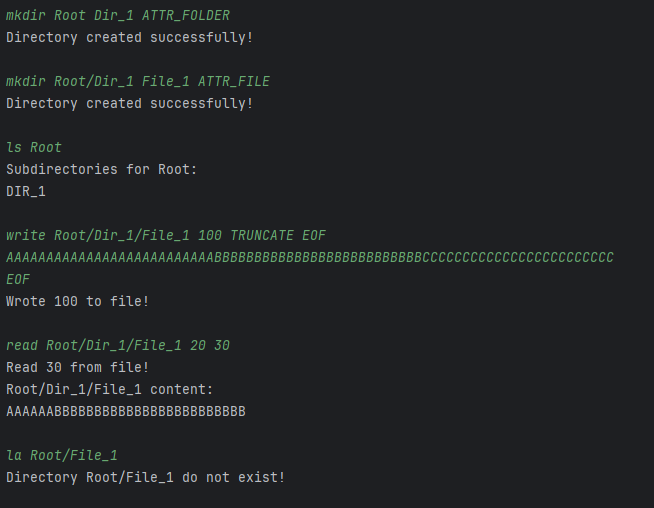
\includegraphics[width=1.0\linewidth]{images/2.5.1.png}
    \label{fig:enter-label}
\end{figure}

\clearpage
\begin{figure}[t!]

    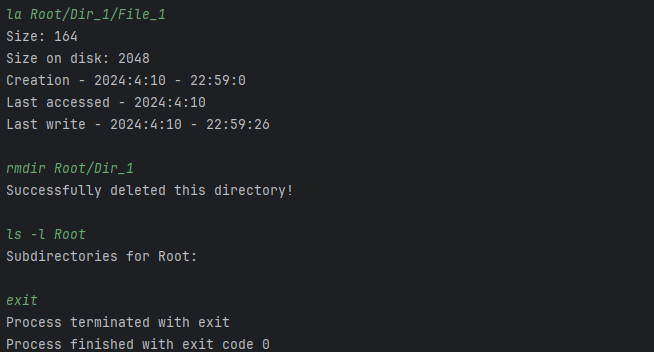
\includegraphics[width=1.0\linewidth]{images/2.5.2.png}
    \label{fig:enter-label}
    \caption{Interacțiunea cu sistemul de fișiere FAT32}
\end{figure}

\bigskip


\subsection{Concluzii FAT32}

În încheiere, FAT32 este un sistem de fișiere relativ simplu, care de-a lungul timpului a dat dovadă de versatilitate și stabilitate, acesta fiind o alegere ideală pentru dispozitivele de stocare de dimensiuni medii. Cu toate acestea, din cauza limitărilor sale, cum ar fi dimensiunea maximă a fișierelor, precum și securității slabe oferite de acesta, FAT32 poate fi neadecvat pentru stocarea unor fișiere de dimensiuni mari, sau pentru gestionarea datelor în siguranță. În concluzie, FAT32 este o alegere ideală datorită compatibilității sale, însă poate fi limitat de anumite caracteristici ale sale.